\documentclass[12pt,a4paper]{article}
\usepackage[utf8]{inputenc}
\usepackage{amsmath}
\usepackage{amsfonts}
\usepackage{amssymb}
\usepackage[none]{hyphenat}
\usepackage{enumerate}
\usepackage[spanish]{babel}
\usepackage{graphicx}
\graphicspath{ {IMAGES/} }
\usepackage{float}
\usepackage{array}
\usepackage{colortbl}
\usepackage{enumitem}
\usepackage{pdfpages}
\usepackage{url, hyperref}
\renewcommand{\arraystretch}{1.8}
\pagestyle{headings}
\author{Juan Sebastian Gonzalez Camacho (1968220), Andrés Felipe Ruíz Buriticá (1968171), Jhoan Sebastian Rojas Holguin (1958337), Carlos Alberto Delgado Galeano (1968127), Jesus Alberto Gil Ayala (1968231)}
\title{Borvo MO - Requirements Specification}
\begin{document}
\begin{titlepage}
\centering
{
\includegraphics[width=0.18 \textwidth]{logo.png} \par}
\vfill
{\bfseries\LARGE Universidad del Valle\par}
{\Large Sede Tuluá\par}
\vfill
{\scshape\Large Ingeniería de Sistemas \par}
\vfill
{\scshape\Huge Borvo - Medicinae Operam \par}
\vfill
{\itshape\Large Taller 2 - Proyecto Final Desarrollo de Software I \par}
\vfill
{\Large Autores: \par}
{\Large Andrés Felipe Ruíz Buriticá - 1968171 \par}
{\Large Carlos Alberto Delgado Galeano - 1968127 \par}
{\Large Jesús Alberto Gil Ayala - 1968231 \par}
{\Large Jhoan Sebastian Rojas Holguin - 1958337 \par}
{\Large Juan Sebastian González Camacho - 1968220 \par}
\vfill
{\Large 15 de Noviembre del 2022 \par}
\end{titlepage}
\tableofcontents
\newpage
\section{Mockups Actualizados}
\begin{figure}[H]
\centering
{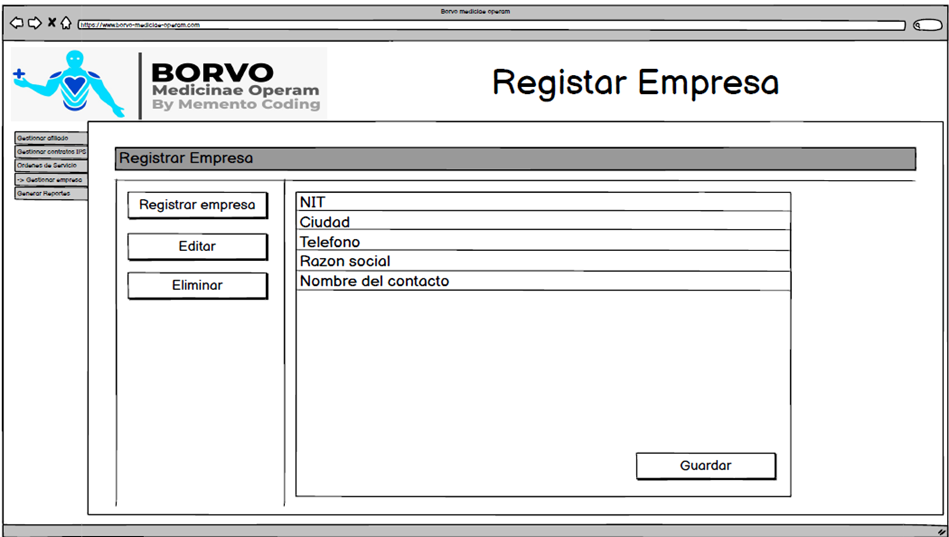
\includegraphics[width=1\textwidth]{Mockup_1.png}\par}
\caption{Mockup Gestionar Empresa}
\end{figure}
\begin{figure}[H]
\centering
{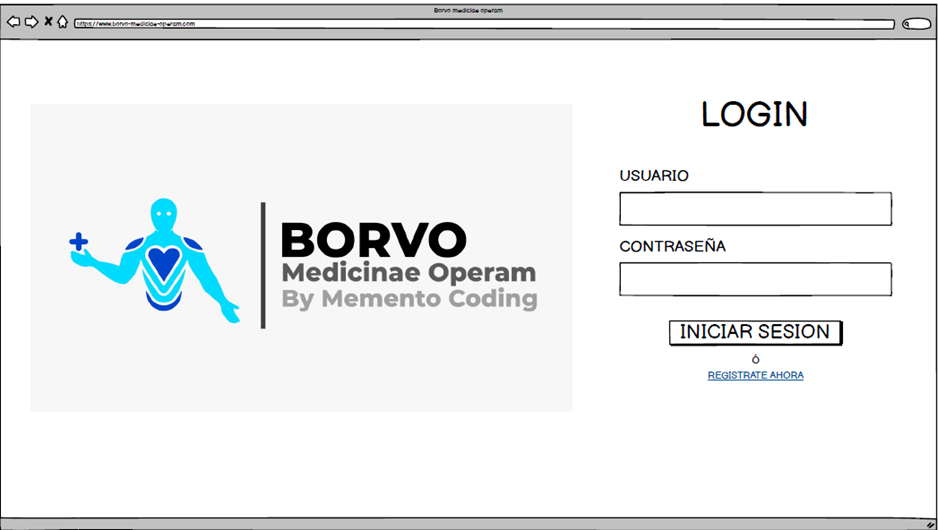
\includegraphics[width=1\textwidth]{Mockup_2.png}\par}
\caption{Mockup Login Cotizante}
\end{figure}
\begin{figure}[H]
\centering
{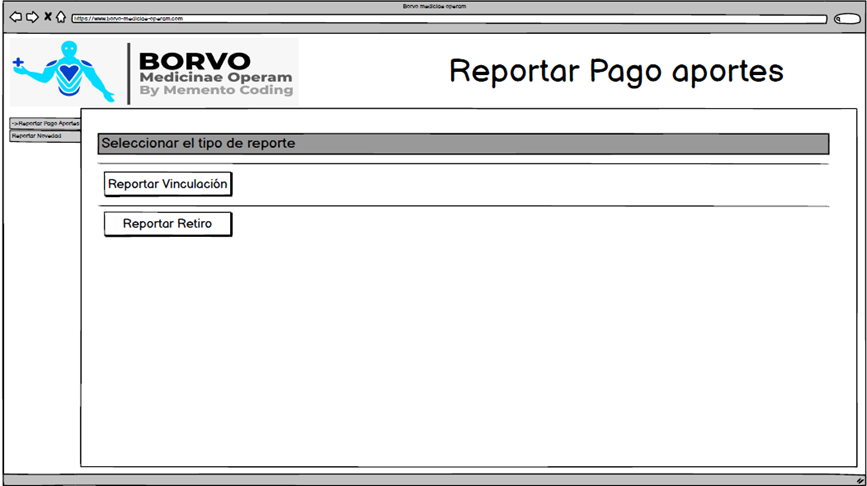
\includegraphics[width=1\textwidth]{Mockup_3.png}\par}
\caption{Mockup Reporte Pago Aportes}
\end{figure}
\begin{figure}[H]
\centering
{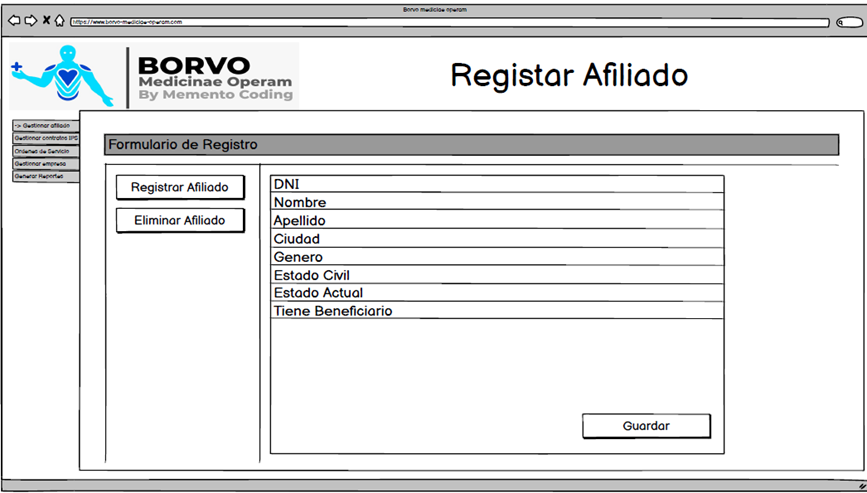
\includegraphics[width=1\textwidth]{Mockup_4.png}\par}
\caption{Mockup Gestionar Afiliado}
\end{figure}
\begin{figure}[H]
\centering
{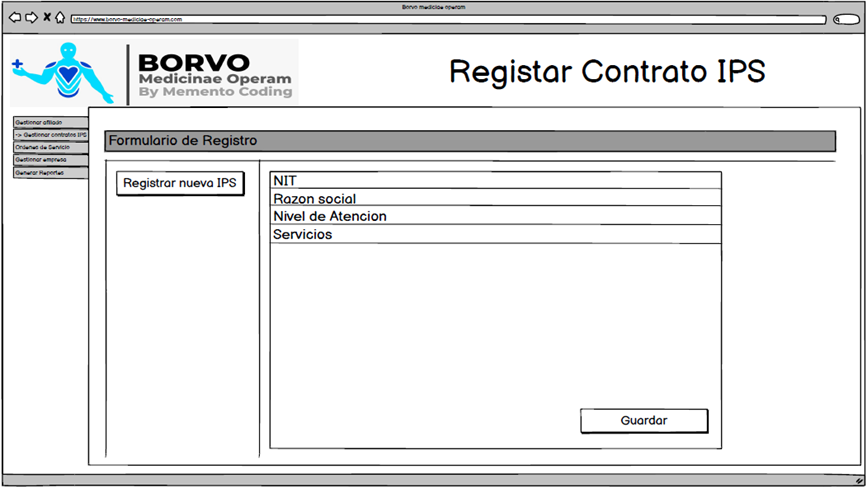
\includegraphics[width=1\textwidth]{Mockup_5.png}\par}
\caption{Mockup Gestionar IPS}
\end{figure}
\begin{figure}[H]
\centering
{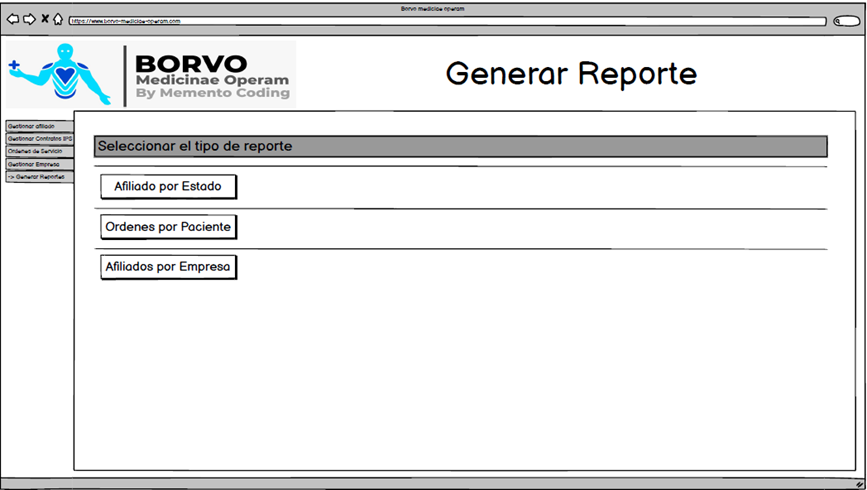
\includegraphics[width=1\textwidth]{Mockup_6.png}\par}
\caption{Mockup Generar Reportes}
\end{figure}
\begin{figure}[H]
\centering
{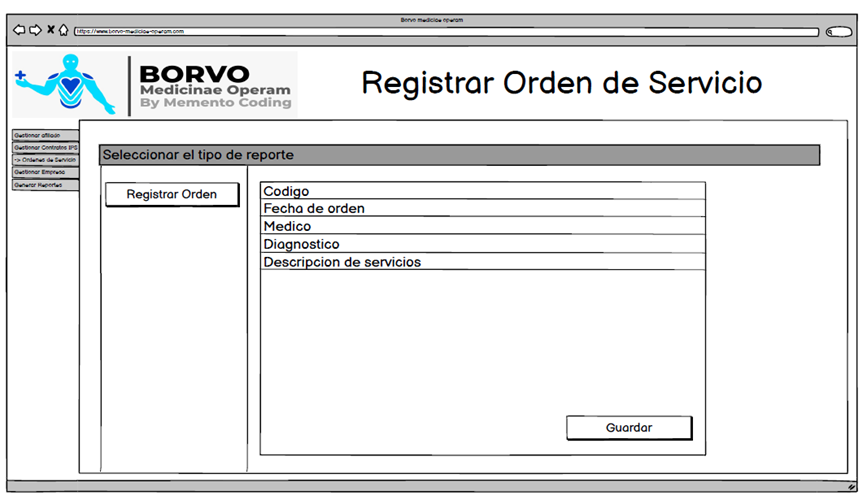
\includegraphics[width=1\textwidth]{Mockup_7.png}\par}
\caption{Mockup Gestionar Orden de Servicio}
\end{figure}
\begin{figure}[H]
\centering
{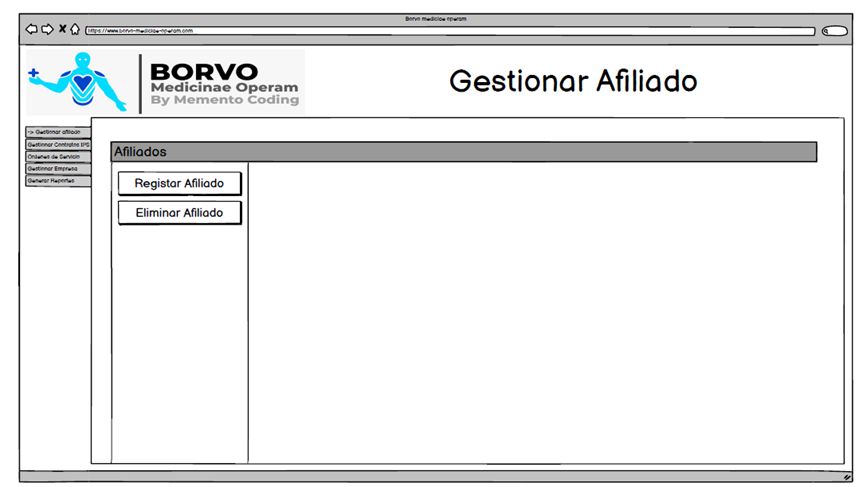
\includegraphics[width=1\textwidth]{Mockup_8.png}\par}
\caption{Mockup Gestionar Afiliado}
\end{figure}
\begin{figure}[H]
\centering
{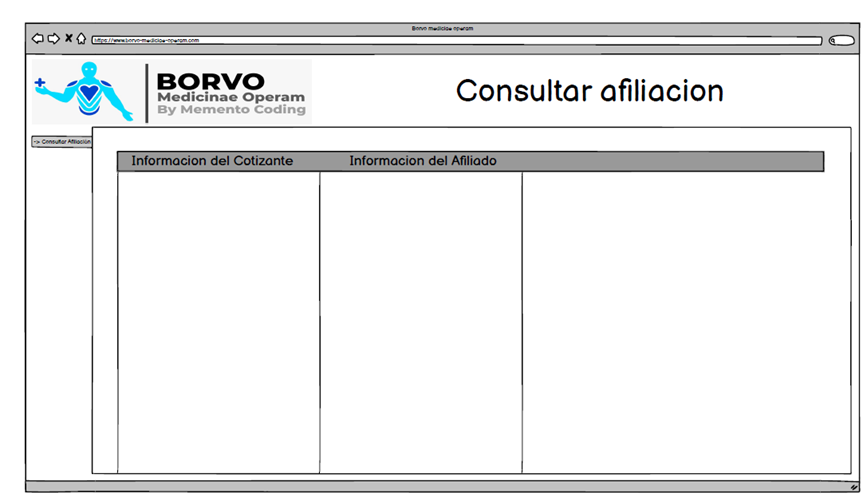
\includegraphics[width=1\textwidth]{Mockup_9.png}\par}
\caption{Mockup Consultar Afiliación}
\end{figure}
\begin{figure}[H]
\centering
{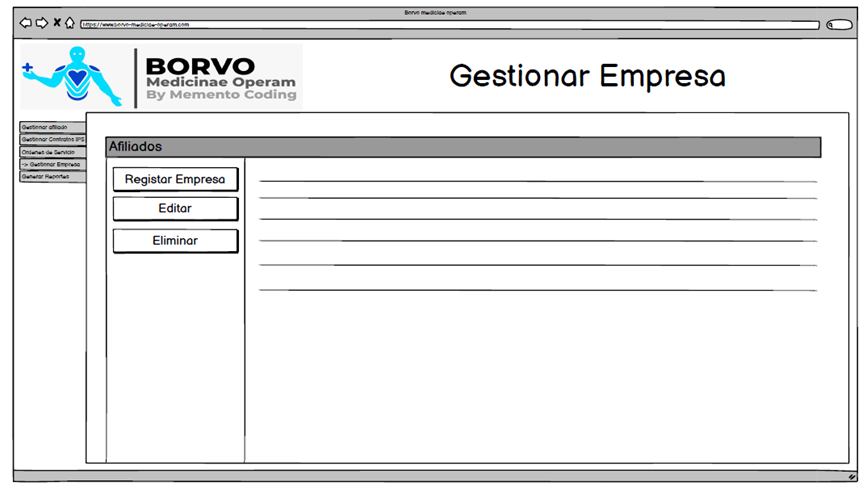
\includegraphics[width=1\textwidth]{Mockup_10.png}\par}
\caption{Mockup Gestionar Empresa}
\end{figure}
\begin{figure}[H]
\centering
{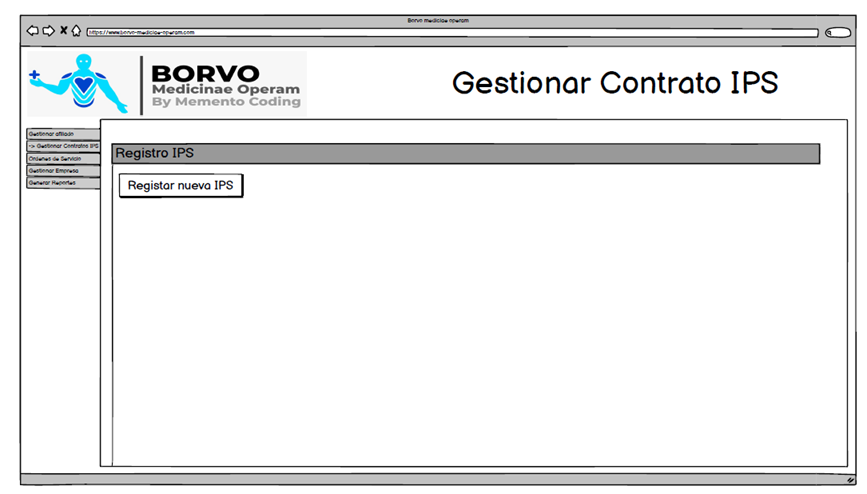
\includegraphics[width=1\textwidth]{Mockup_11.png}\par}
\caption{Mockup Gestionar IPS}
\end{figure}
\begin{figure}[H]
\centering
{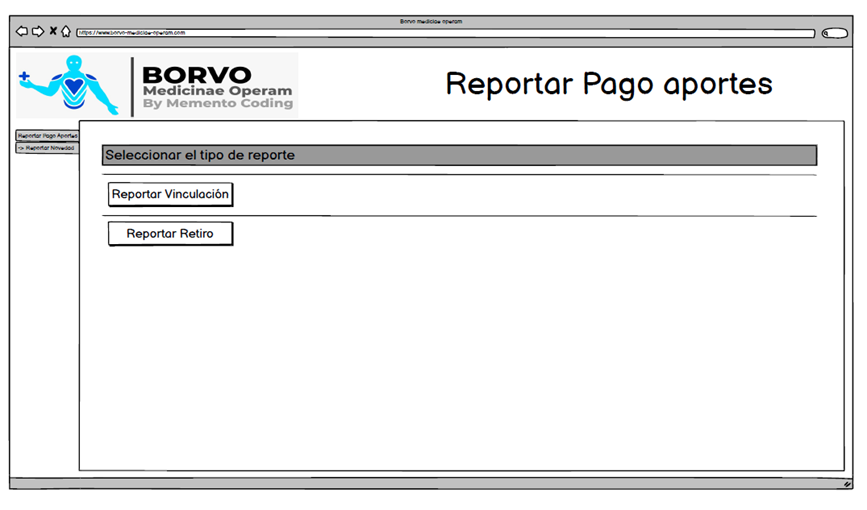
\includegraphics[width=1\textwidth]{Mockup_12.png}\par}
\caption{Mockup Reportar Novedad}
\end{figure}
\section{Artefactos Ágiles}
\subsection{Roles Equipo Scrum}
\begin{center}
\begin{tabular}{|m{5cm}|m{9cm}|}
\hline
\textbf{Rol} & Product Owner. \\
\hline
\textbf{Integrante Asignado} & Juan Sebastian Gonzalez Camacho. \\
\hline
\textbf{Descripción del Rol} & El Product Owner es el encargado de optimizar y maximizar el valor del producto, siendo la persona encargada de gestionar el flujo de valor del producto a través del Product Backlog. \\
\hline
\textbf{Funciones del Rol} & \begin{enumerate}[noitemsep]
								 \item Definir los objetivos del producto.
								 \item Determinar las características del producto.
								 \item Crear el Backlog.
								 \item Crear Historias de Usuario.
								 \item Priorizar y gestionar el Backlog.
								 \item Supervizar las etapas de desarrollo del producto.	
							\end{enumerate} \\
\hline
\end{tabular}
\vspace{5mm}

\begin{tabular}{|m{5cm}|m{9cm}|}
\hline
\textbf{Rol} & Scrum Master. \\
\hline
\textbf{Integrante Asignado} & Andres Felipe Ruiz Buritica. \\
\hline
\textbf{Descripción del Rol} & El Scrum Master se encarga de gestionar el proceso Scrum y ayudar a eliminar impedimentos que puedan afectar a la entrega del producto. Además, se encarga de las labores de mentoring y formación, coaching y de facilitar reuniones y eventos si es necesario. \\
\hline
\textbf{Funciones del Rol} & \begin{enumerate}[noitemsep]
								 \item Gestionar el proceso.
								 \item Eliminar impedimentos.
								 \item Planear reuniones.
								 \item Dirigir al equipo de desarrollo.	
							\end{enumerate} \\
\hline
\end{tabular}
\vspace{5mm}

\begin{tabular}{|m{5cm}|m{9cm}|}
\hline
\textbf{Rol} & Equipo de Desarrollo. \\
\hline
\textbf{Integrante Asignado} & Carlos Alberto Delgado Galeano, Jesus Alberto Gil Ayala, Jhoan Sebastian Rojas Holguin. \\
\hline
\textbf{Descripción del Rol} & El equipo de desarrollo suele estar formado por entre 3 a 9 profesionales que se encargan de desarrollar el producto, auto-organizándose y auto-gestionándose para conseguir entregar un incremento de software al final del ciclo de desarrollo. \\
\hline
\textbf{Funciones del Rol} & \begin{enumerate}[noitemsep]
								 \item Desarrollar el producto.
								 \item Revisar el Backlog y los Sprint Plan.
								 \item Entregar las tareas terminadas.
								 \item Comunicarse constantemente con el Scrum Master.	
							\end{enumerate} \\
\hline
\end{tabular}
\vspace{5mm}


\end{center}
\newpage
\subsection{Sprint 0}
\begin{enumerate}
\item Levantamiento de requerimientos funcionales y no funcionales.
\item Elaboración del diagrama de casos de uso y especificación de casos de uso.
\item Diseño del modelo entidad relación y modelo relacional.
\item Diseño del diagrama de clases.
\item Asignación de roles Scrum.
\item Elaboración del User Story Mapping.
\item Redacción de Historias de Usuario.
\item Diseño del Backlog.
\item Elaboración del Release Plan.
\item Elaboración del Sprint Plan.
\item Cronograma de ceremonias ágiles.
\item Elección de herramientas, gestores, frameworks y demás elementos a utilizar.
\end{enumerate}
\subsection{User Story Mapping}
\begin{figure}[H]
\centering
{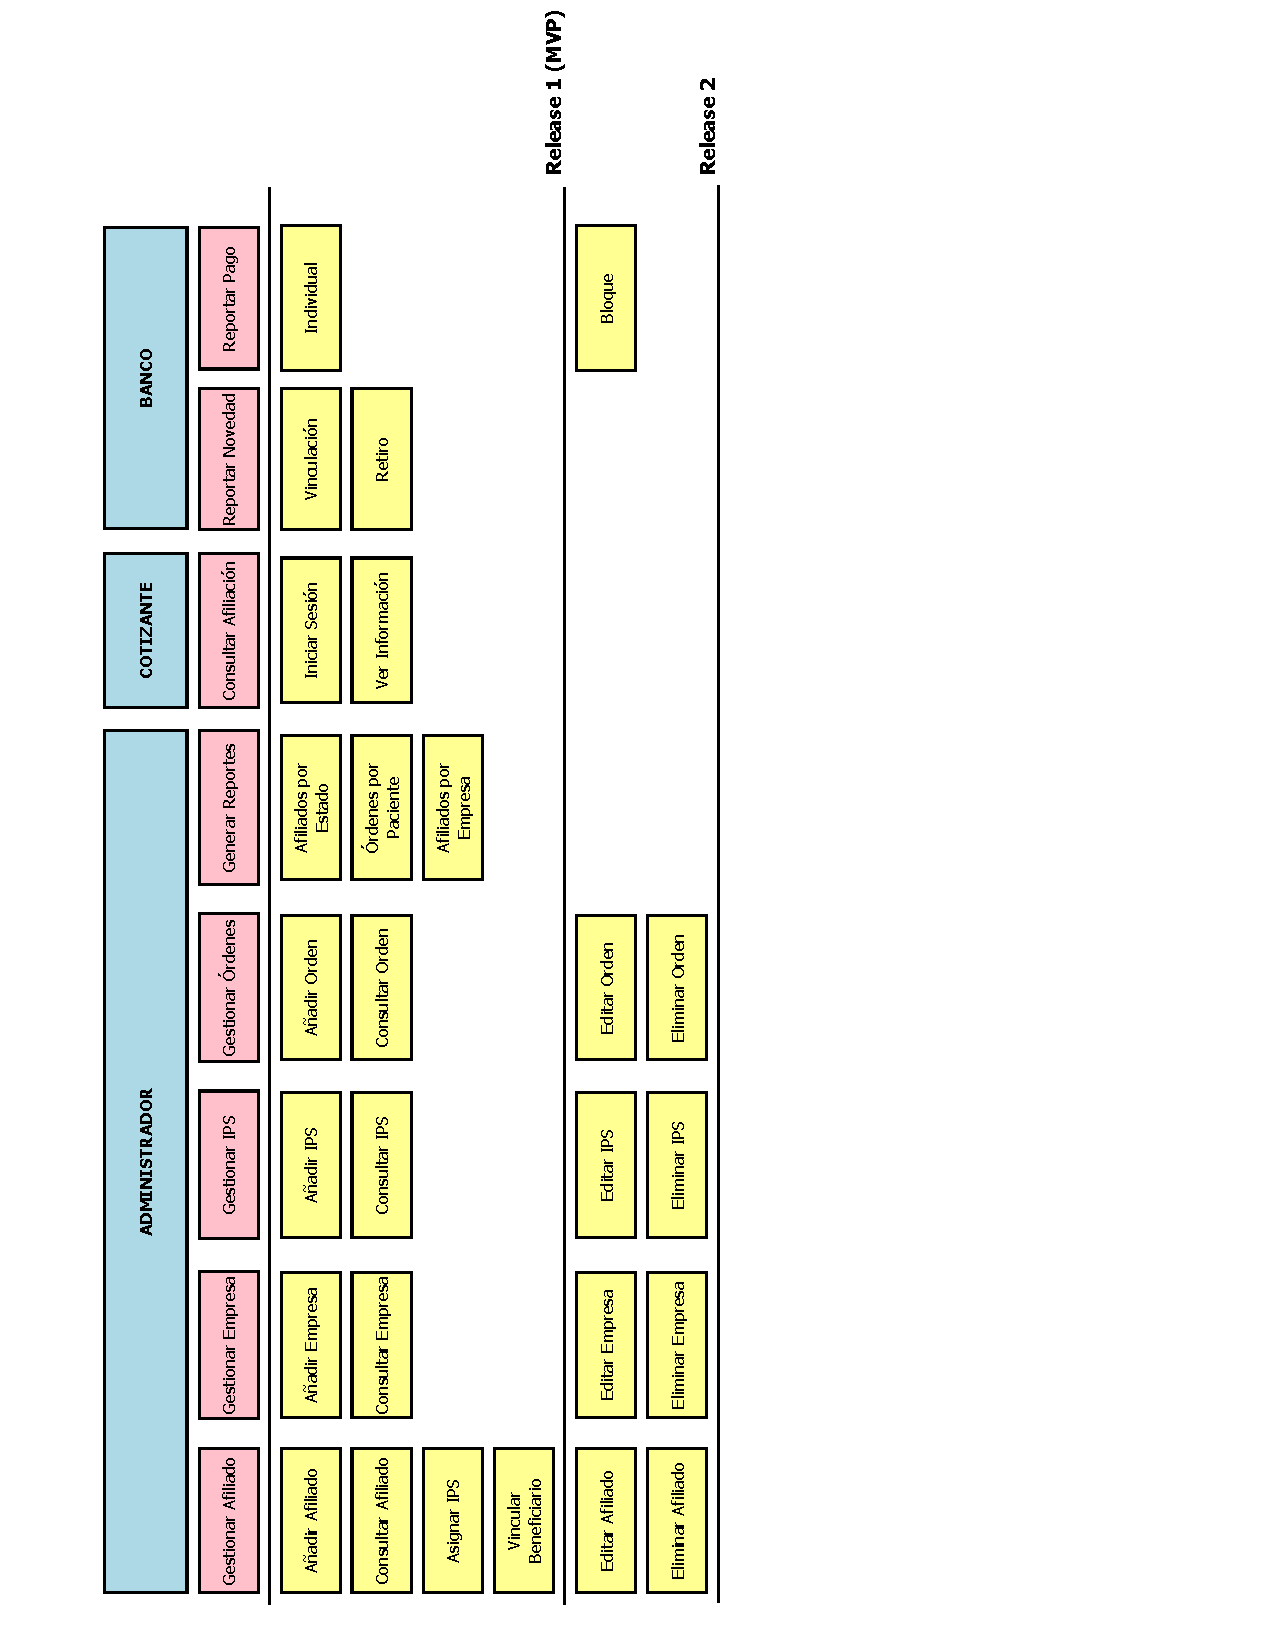
\includegraphics[width=0.8\textwidth, angle=-90]{User_Story_Mapping.pdf} \par}
\caption{User Story Mapping}
\end{figure}
\newpage
\subsection{Historias de Usuario}
\begin{center}
\begin{tabular}{|>{\columncolor[RGB]{215, 215, 215}} p{10cm} >{\columncolor[RGB]{215, 215, 215}} c >{\columncolor[RGB]{215, 215, 215}} p{2.5cm}|}
\hline 
\textbf{Historia de Usuario \#1}

Gestionar afiliados & & \textbf{{\Large EPIC}} \\ 
\textbf{Descripción}

Como administrador, quiero gestionar la información de los afiliados, para poder mantener los datos actualizados en el sistema. &  & \textbf{Prioridad}

Alta\\

\textbf{Criterio de Aceptación}

\begin{itemize}
\item Dado que una afiliado no existe en el sistema, cuando el administrador lo registra, entonces el sistema muestra un mensaje indicando que la operación ha sido exitosa.
\item Dado que un afiliado tiene beneficiarios, cuando el administrador los registra, entonces el sistema muestra un mensaje indicando que la operación ha sido un éxito.
\item Dado que un afiliado tiene distintos datos, cuando el administrador ve los detalles, entonces el sistema muestra una página con toda la información del cotizante, incluyendo sus beneficiarios.
\item Dado que un afiliado tiene información desactualizada, cuando el administrador la edita, entonces el sistema muestra un formulario de edición y al final un mensaje indicando que los datos han sido modificados.
\item Dado que un afiliado ya no tiene relación con la EPS, cuando el administrador lo elimina, el sistema desactiva la cuenta y muestra un mensaje de éxito.
\end{itemize} & & \textbf{Estimación}

13 \\ 
\hline 
\end{tabular}
\vspace{5mm}

\begin{tabular}{| p{10cm} c p{2.5cm}|}
\hline 
\textbf{Historia de Usuario \#2}

Ver información de un afiliado & & \textbf{{\Large STORY}} \\ 
\textbf{Descripción}

Como administrador, quiero ver los datos de un cotizante y sus beneficiarios, para poder saber qué información contiene el sistema sobre ellos. &  & \textbf{Prioridad}

Alta\\

\textbf{Criterio de Aceptación}

\begin{itemize}
\item Dado que existen distintos cotizantes, cuando el administrador accede a los detalles de alguno, el sistema le muestra una página con toda la información relacionada del cotizante y sus beneficiarios.
\end{itemize} & & \textbf{Estimación}

5 \\ 
\hline 
\end{tabular}
\vspace{5mm}

\begin{tabular}{| p{10cm} c p{2.5cm}|}
\hline 
\textbf{Historia de Usuario \#3}

Añadir afiliados & & \textbf{{\Large STORY}} \\ 
\textbf{Descripción}

Como administrador, quiero añadir un cotizante y sus beneficiarios, para
poder gestionar su información posteriormente. &  & \textbf{Prioridad}

Alta\\

\textbf{Criterio de Aceptación}

\begin{itemize}
\item Dado que el cotizante no existe en el sistema, cuando el
administrador lo añade, entonces el sistema le muestra una
notificación indicando que la operación ha sido exitosa.
\item Dado que el cotizante y/o beneficiario ya existe en el sistema,
cuando el administrador lo añade, entonces el sistema le
muestra una notificación indicando que ya existe.
\end{itemize} & & \textbf{Estimación}

5 \\ 
\hline 
\end{tabular}
\vspace{5mm}

\begin{tabular}{| p{10cm} c p{2.5cm}|}
\hline 
\textbf{Historia de Usuario \#4}

Editar afiliados & & \textbf{{\Large STORY}} \\ 
\textbf{Descripción}

Como administrador, quiero editar la información de un cotizante y sus
beneficiarios, para poder mantener actualizado el registro de ellos en el
sistema. &  & \textbf{Prioridad}

Alta\\

\textbf{Criterio de Aceptación}

\begin{itemize}
\item Dado que un afiliado tiene información desactualizada, cuando el
administrador edita sus datos, entonces el sistema le muestra
una notificación indicando que el registro se ha actualizado.
\end{itemize} & & \textbf{Estimación}

5 \\ 
\hline 
\end{tabular}
\vspace{5mm}

\begin{tabular}{| p{10cm} c p{2.5cm}|}
\hline 
\textbf{Historia de Usuario \#5}

Eliminar afiliados & & \textbf{{\Large STORY}} \\ 
\textbf{Descripción}

Como administrador, quiero eliminar un cotizante que ya no tiene
contrato junto con sus beneficiarios, para poder mantener el registro del
sistema actualizado. &  & \textbf{Prioridad}

Alta\\

\textbf{Criterio de Aceptación}

\begin{itemize}
\item Dado que un cotizante ya no tiene relación con la EPS, cuando el
administrador la elimina, entonces el sistema elimina también a
sus beneficiarios y muestra una notificación señalando que la
operación ha sido exitosa.
\end{itemize} & & \textbf{Estimación}

5 \\ 
\hline 
\end{tabular}
\vspace{5mm}

\begin{tabular}{|>{\columncolor[RGB]{215, 215, 215}} p{10cm} >{\columncolor[RGB]{215, 215, 215}} c >{\columncolor[RGB]{215, 215, 215}} p{2.5cm}|}
\hline 
\textbf{Historia de Usuario \#6}

Gestionar IPS & & \textbf{{\Large EPIC}} \\ 
\textbf{Descripción}

Como administrador, quiero gestionar los contratos de las IPS, para poder
mantener el registro del sistema actualizado. &  & \textbf{Prioridad}

Alta\\

\textbf{Criterio de Aceptación}

\begin{itemize}
\item Dado que una IPS no existe en el sistema, cuando el
administrador la añade, entonces el sistema muestra un mensaje
indicando que la operación ha sido exitosa.
\item Dado que hay muchas IPS en el sistema, cuando el administrador
intenta ver los detalles de alguna, el sistema le muestra toda la
información guardada relacionada.
\item Dado que una IPS ya no tiene contrato con la EPS, cuando el
administrador la elimina, entonces el sistema muestra un
mensaje indicando que la operación ha sido exitosa.
\item Dado que los datos de una IPS han cambiado, cuando el
administrador intenta editarla, el sistema le muestra un
formulación de edición y al terminar, un mensaje indicando que
la operación ha sido exitosa.
\end{itemize} & & \textbf{Estimación}

8 \\ 
\hline 
\end{tabular}
\vspace{5mm}

\begin{tabular}{| p{10cm} c p{2.5cm}|}
\hline 
\textbf{Historia de Usuario \#7}

Ver información de una IPS & & \textbf{{\Large STORY}} \\ 
\textbf{Descripción}

Como administrador, quiero ver los datos de una IPS, para poder saber
qué información contiene el sistema sobre ella. &  & \textbf{Prioridad}

Alta\\

\textbf{Criterio de Aceptación}

\begin{itemize}
\item Dado que existen distintas IPS, cuando el administrador accede a
los detalles de alguna, el sistema le muestra una página con toda
la información relacionada.
\end{itemize} & & \textbf{Estimación}

3 \\ 
\hline 
\end{tabular}
\vspace{5mm}

\begin{tabular}{| p{10cm} c p{2.5cm}|}
\hline 
\textbf{Historia de Usuario \#8}

Añadir IPS & & \textbf{{\Large STORY}} \\ 
\textbf{Descripción}

Como administrador, quiero añadir un contrato con una IPS, para poder
gestionar las órdenes de servicio que ella ofrece. &  & \textbf{Prioridad}

Alta\\

\textbf{Criterio de Aceptación}

\begin{itemize}
\item Dado que la IPS no existe en el sistema, cuando el administrador
la añade, entonces el sistema le muestra una notificación
indicando que la operación ha sido exitosa.
\item Dado que la IPS ya existe en el sistema, cuando el administrador
la añade, entonces el sistema le muestra una notificación
indicando que ya existe otra IPS con el mismo NIT y razón social.
\end{itemize} & & \textbf{Estimación}

3 \\ 
\hline 
\end{tabular}
\vspace{5mm}

\begin{tabular}{| p{10cm} c p{2.5cm}|}
\hline 
\textbf{Historia de Usuario \#9}

Editar IPS & & \textbf{{\Large STORY}} \\ 
\textbf{Descripción}

Como administrador, quiero editar la información de una IPS, para poder
mantener actualizado el registro de ella en el sistema. &  & \textbf{Prioridad}

Alta\\

\textbf{Criterio de Aceptación}

\begin{itemize}
\item Dado que una IPS tiene información desactualizada, cuando el
administrador edita sus datos, entonces el sistema le muestra
una notificación indicando que el registro se ha actualizado.
\end{itemize} & & \textbf{Estimación}

3 \\ 
\hline 
\end{tabular}
\vspace{5mm}

\begin{tabular}{| p{10cm} c p{2.5cm}|}
\hline 
\textbf{Historia de Usuario \#10}

Eliminar IPS & & \textbf{{\Large STORY}} \\ 
\textbf{Descripción}

Como administrador, quiero eliminar una IPS que ya no tiene contrato,
para poder mantener el registro del sistema actualizado. &  & \textbf{Prioridad}

Alta\\

\textbf{Criterio de Aceptación}

\begin{itemize}
\item Dado que una IPS ya no tiene relación con la EPS, cuando el
administrador la elimina, entonces el sistema muestra una
notificación señalando que la operación ha sido exitosa.
\end{itemize} & & \textbf{Estimación}

3 \\ 
\hline 
\end{tabular}
\vspace{5mm}

\begin{tabular}{|>{\columncolor[RGB]{215, 215, 215}} p{10cm} >{\columncolor[RGB]{215, 215, 215}} c >{\columncolor[RGB]{215, 215, 215}} p{2.5cm}|}
\hline 
\textbf{Historia de Usuario \#11}

Gestionar empresa & & \textbf{{\Large EPIC}} \\ 
\textbf{Descripción}


Como administrador, quiero gestionar la información de las empresas,
para poder mantener el registro del sistema actualizado. &  & \textbf{Prioridad}

Alta\\

\textbf{Criterio de Aceptación}

\begin{itemize}
\item Dado que una empresa no existe en el sistema, cuando el
administrador la añade, entonces el sistema muestra un mensaje
indicando que la operación ha sido exitosa.
\item Dado que hay muchas empresas en el sistema, cuando el
administrador intenta ver los detalles de alguna, el sistema le
muestra toda la información guardada relacionada.
\item Dado que una empresa ya no tiene relación con el EPS, cuando el
administrador la elimina, entonces el sistema muestra un
mensaje indicando que la operación ha sido exitosa.
\item Dado que la información de una empresa ha cambiado, cuando
el administrador intenta editarla, el sistema le muestra un
formulación de edición y al terminar, un mensaje indicando que
la operación ha sido exitosa.
\end{itemize} & & \textbf{Estimación}

8 \\ 
\hline 
\end{tabular}
\vspace{5mm}

\begin{tabular}{| p{10cm} c p{2.5cm}|}
\hline 
\textbf{Historia de Usuario \#12}

Ver información de una empresa & & \textbf{{\Large STORY}} \\ 
\textbf{Descripción}

Como administrador, quiero ver la información de una empresa, para
poder saber qué información contiene el sistema sobre ella. &  & \textbf{Prioridad}

Alta\\

\textbf{Criterio de Aceptación}

\begin{itemize}
\item Dado que existen distintas empresas, cuando el administrador
accede a los detalles de alguna, el sistema le muestra una página
con toda la información relacionada.
\end{itemize} & & \textbf{Estimación}

3 \\ 
\hline 
\end{tabular}
\vspace{5mm}

\begin{tabular}{| p{10cm} c p{2.5cm}|}
\hline 
\textbf{Historia de Usuario \#13}

Añadir empresa & & \textbf{{\Large STORY}} \\ 
\textbf{Descripción}

Como administrador, quiero añadir nuevas empresas al sistema, para
poder gestionar los afiliados que pertenezcan a ella. &  & \textbf{Prioridad}

Alta\\

\textbf{Criterio de Aceptación}

\begin{itemize}
\item Dado que la empresa no existe en el sistema, cuando el
administrador la añade, entonces el sistema le muestra una
notificación indicando que la operación ha sido exitosa.
\item Dado que la empresa ya existe en el sistema, cuando el
administrador la añade, entonces el sistema le muestra una
notificación indicando que ya existe otra empresa con el mismo
NIT y razón social.
\end{itemize} & & \textbf{Estimación}

3 \\ 
\hline 
\end{tabular}
\vspace{5mm}

\begin{tabular}{| p{10cm} c p{2.5cm}|}
\hline 
\textbf{Historia de Usuario \#14}

Editar empresa & & \textbf{{\Large STORY}} \\ 
\textbf{Descripción}

Como administrador, quiero editar la información de una empresa, para
poder mantener actualizado el registro de empresas del sistema. &  & \textbf{Prioridad}

Alta\\

\textbf{Criterio de Aceptación}

\begin{itemize}
\item Dado que una empresa tiene información desactualizada, cuando
el administrador edita sus datos, entonces el sistema le muestra
una notificación indicando que el registro se ha actualizado.
\end{itemize} & & \textbf{Estimación}

3 \\ 
\hline 
\end{tabular}
\vspace{5mm}

\begin{tabular}{| p{10cm} c p{2.5cm}|}
\hline 
\textbf{Historia de Usuario \#15}

Eliminar empresa & & \textbf{{\Large STORY}} \\ 
\textbf{Descripción}

Como administrador, quiero eliminar una empresa del sistema, para
poder mantener el registro del sistema actualizado. &  & \textbf{Prioridad}

Alta\\

\textbf{Criterio de Aceptación}

\begin{itemize}
\item Dado que una empresa ya no tiene relación con la EPS, cuando el
administrador la elimina, entonces el sistema muestra una
notificación señalando que la operación ha sido exitosa.
\end{itemize} & & \textbf{Estimación}

3 \\ 
\hline 
\end{tabular}
\vspace{5mm}

\begin{tabular}{|>{\columncolor[RGB]{215, 215, 215}} p{10cm} >{\columncolor[RGB]{215, 215, 215}} c >{\columncolor[RGB]{215, 215, 215}} p{2.5cm}|}
\hline 
\textbf{Historia de Usuario \#16}

Reportar novedad & & \textbf{{\Large EPIC}} \\ 
\textbf{Descripción}

Como banco registrado en el sistema, quiero reportar la vinculación o
retiro de un empleado, para poder activar o desactivar la cuenta del
cotizante dentro del sistema. &  & \textbf{Prioridad}

Alta\\

\textbf{Criterio de Aceptación}

\begin{itemize}
\item Dado que el empleado se retiró de la empresa, cuando el banco
reporta su retiro, entonces el sistema cambia el estado del
cotizante a retirado e inactiva la cuenta de usuario asociada.
\item Dado que el empleado se vinculó a la empresa, cuando el banco
reporta su vinculación, entonces el sistema crea su cuenta.
\end{itemize} & & \textbf{Estimación}

5 \\ 
\hline 
\end{tabular}
\vspace{5mm}

\begin{tabular}{| p{10cm} c p{2.5cm}|}
\hline 
\textbf{Historia de Usuario \#17}

Reportar vinculación de cotizante & & \textbf{{\Large STORY}} \\ 
\textbf{Descripción}

Como banco registrado en el sistema, quiero reportar la vinculación de
un empleado, para poder activar la cuenta del cotizante dentro del
sistema. &  & \textbf{Prioridad}

Alta\\

\textbf{Criterio de Aceptación}

\begin{itemize}
\item Dado que el empleado se vinculó a la empresa, cuando el banco
reporta su vinculación, entonces el sistema crea su cuenta.
\end{itemize} & & \textbf{Estimación}

3 \\ 
\hline 
\end{tabular}
\vspace{5mm}

\begin{tabular}{| p{10cm} c p{2.5cm}|}
\hline 
\textbf{Historia de Usuario \#18}

Reportar retiro de cotizante & & \textbf{{\Large STORY}} \\ 
\textbf{Descripción}

Como banco registrado en el sistema, quiero reportar el retiro de un
empleado, para poder desactivar la cuenta del cotizante dentro del
sistema. &  & \textbf{Prioridad}

Alta\\

\textbf{Criterio de Aceptación}

\begin{itemize}
\item Dado que el empleado se retiró de la empresa, cuando el banco
reporta su retiro, entonces el sistema cambia el estado del
cotizante a retirado e inactiva la cuenta de usuario asociada.
\end{itemize} & & \textbf{Estimación}

3 \\ 
\hline 
\end{tabular}
\vspace{5mm}

\begin{tabular}{|>{\columncolor[RGB]{215, 215, 215}} p{10cm} >{\columncolor[RGB]{215, 215, 215}} c >{\columncolor[RGB]{215, 215, 215}} p{2.5cm}|}
\hline 
\textbf{Historia de Usuario \#19}

Generar reportes & & \textbf{{\Large EPIC}} \\ 
\textbf{Descripción}

Como administrador, quiero generar distintos reportes, para poder ver la
información actual que contiene el sistema. &  & \textbf{Prioridad}

Media\\

\textbf{Criterio de Aceptación}

\begin{itemize}
\item Dado que hay afiliados con distinto estado, cuando el
administrador genera el reporte, entonces el sistema le muestra
una lista de todos los afiliados con el estado actual de ellos.
\item Dado que hay órdenes de servicio por pacientes, cuando el
administrador genera el reporte, entonces el sistema le muestra
una lista de todos los afiliados con las órdenes de servicios que
han sacado hasta la fecha.
\item Dado que hay cotizantes por empresa, cuando el administrador
genera el reporte, entonces el sistema muestra una lista de todos
los afiliados junto con la información de la empresa a la que
perteneces.
\end{itemize} & & \textbf{Estimación}

2 \\ 
\hline 
\end{tabular}
\vspace{5mm}

\begin{tabular}{| p{10cm} c p{2.5cm}|}
\hline 
\textbf{Historia de Usuario \#20}

Generar reporte de afiliados por estado & & \textbf{{\Large STORY}} \\ 
\textbf{Descripción}

Como administrador, quiero generar un reporte de afiliados por estado,
para poder ver la información actual que contiene el sistema. &  & \textbf{Prioridad}

Media\\

\textbf{Criterio de Aceptación}

\begin{itemize}
\item Dado que hay afiliados con distinto estado, cuando el
administrador genera el reporte, entonces el sistema le muestra
una lista de todos los afiliados con el estado actual de ellos.
\end{itemize} & & \textbf{Estimación}

2 \\ 
\hline 
\end{tabular}
\vspace{5mm}

\begin{tabular}{| p{10cm} c p{2.5cm}|}
\hline 
\textbf{Historia de Usuario \#21}

Generar reporte de órdenes de servicio por paciente & & \textbf{{\Large STORY}} \\ 
\textbf{Descripción}

Como administrador, quiero generar reportes de órdenes de servicio por
paciente, para poder ver la información actual que contiene el sistema. &  & \textbf{Prioridad}

Media\\

\textbf{Criterio de Aceptación}

\begin{itemize}
\item Dado que hay órdenes de servicio por pacientes, cuando el
administrador genera el reporte, entonces el sistema le muestra
una lista de todos los afiliados con las órdenes de servicios que
han sacado hasta la fecha.
\end{itemize} & & \textbf{Estimación}

2 \\ 
\hline 
\end{tabular}
\vspace{5mm}

\begin{tabular}{| p{10cm} c p{2.5cm}|}
\hline 
\textbf{Historia de Usuario \#22}

Generar reportes de cotizantes por empresa & & \textbf{{\Large STORY}} \\ 
\textbf{Descripción}

Como administrador, quiero generar reportes de cotizantes por empresa,
para poder ver la información actual que contiene el sistema. &  & \textbf{Prioridad}

Media\\

\textbf{Criterio de Aceptación}

\begin{itemize}
\item Dado que hay cotizantes por empresa, cuando el administrador
genera el reporte, entonces el sistema muestra una lista de todos
los afiliados junto con la información de la empresa a la que
perteneces.
\end{itemize} & & \textbf{Estimación}

2 \\ 
\hline 
\end{tabular}
\vspace{5mm}

\begin{tabular}{|>{\columncolor[RGB]{215, 215, 215}} p{10cm} >{\columncolor[RGB]{215, 215, 215}} c >{\columncolor[RGB]{215, 215, 215}} p{2.5cm}|}
\hline 
\textbf{Historia de Usuario \#23}

Reportar pago de aportes & & \textbf{{\Large EPIC}} \\ 
\textbf{Descripción}

Como banco registrado en el sistema, quiero reportar el pago de
cotizantes, para poder mantener la información financiera actualizada
cada mes. &  & \textbf{Prioridad}

Alta\\

\textbf{Criterio de Aceptación}

\begin{itemize}
\item Dado que hay pagos de muchos cotizantes por reportar, cuando
el banco solicita hacer el reporte, entonces el sistema le muestra
un formulario por cada cotizante.
\item Dado que hay pagos de un cotizante por reportar, cuando el
banco solicita hacer el reporte, entonces el sistema le muestra un
formulario para el cotizante.
\item Dado que el banco está llenando la información del reporte,
cuando ingresa mal algún dato, entonces el sistema le notifica el
error para corregirlo.
\end{itemize} & & \textbf{Estimación}

5 \\ 
\hline 
\end{tabular}
\vspace{5mm}

\begin{tabular}{| p{10cm} c p{2.5cm}|}
\hline 
\textbf{Historia de Usuario \#24}

Reportar pago de aportes individual & & \textbf{{\Large STORY}} \\ 
\textbf{Descripción}

Como banco registrado en el sistema, quiero reportar el pago de aportes
de cotizantes de forma individual, para poder registrar uno por uno
manualmente cuando sean muy pocos. &  & \textbf{Prioridad}

Alta\\

\textbf{Criterio de Aceptación}

\begin{itemize}
\item Dado que hay empresas que hacen pocos pagos de aportes, cuando el banco solicita
hacer el reporte, entonces el sistema le permite registrarlos de forma individual
mediante un formulario.
\end{itemize} & & \textbf{Estimación}

3 \\ 
\hline 
\end{tabular}
\vspace{5mm}

\begin{tabular}{| p{10cm} c p{2.5cm}|}
\hline 
\textbf{Historia de Usuario \#25}

Reportar pago de aportes en bloque & & \textbf{{\Large STORY}} \\ 
\textbf{Descripción}

Como banco registrado en el sistema, quiero reportar los pagos de aportes
de los cotizantes de una empresa en bloque, para poder registrar con mayor
agilidad cuando sean reportados muchos pagos. &  & \textbf{Prioridad}

Media\\

\textbf{Criterio de Aceptación}

\begin{itemize}
\item Dado que hay empresas que reportan muchos pagos, cuando el banco solicita
hacer el reporte, el sistema le permite cargar desde un archivo varios reportes.
\end{itemize} & & \textbf{Estimación}

3 \\ 
\hline 
\end{tabular}
\vspace{5mm}

\begin{tabular}{|>{\columncolor[RGB]{215, 215, 215}} p{10cm} >{\columncolor[RGB]{215, 215, 215}} c >{\columncolor[RGB]{215, 215, 215}} p{2.5cm}|}
\hline 
\textbf{Historia de Usuario \#26}

Gestionar orden de servicio & & \textbf{{\Large EPIC}} \\ 
\textbf{Descripción}


Como administrador, quiero gestionar la información de las órdenes de servicio,
para poder mantener el registro del sistema actualizado. &  & \textbf{Prioridad}

Alta\\

\textbf{Criterio de Aceptación}

\begin{itemize}
\item Dado que una orden de servicio no existe en el sistema, cuando el
administrador la añade, entonces el sistema muestra un mensaje
indicando que la operación ha sido exitosa.
\item Dado que hay muchas órdenes de servicio en el sistema, cuando el
administrador intenta ver los detalles de alguna, el sistema le
muestra toda la información guardada relacionada.
\item Dado que una órden de servicio ya no tiene relación con el EPS, cuando el
administrador la elimina, entonces el sistema muestra un
mensaje indicando que la operación ha sido exitosa.
\item Dado que la información de una órden de servicio ha cambiado, cuando
el administrador intenta editarla, el sistema le muestra un
formulación de edición y al terminar, un mensaje indicando que
la operación ha sido exitosa.
\end{itemize} & & \textbf{Estimación}

8 \\ 
\hline 
\end{tabular}
\vspace{5mm}

\begin{tabular}{| p{10cm} c p{2.5cm}|}
\hline 
\textbf{Historia de Usuario \#27}

Ver información de una orden de servicio & & \textbf{{\Large STORY}} \\ 
\textbf{Descripción}

Como administrador, quiero ver la información de una orden de servicio, para
poder saber qué información contiene el sistema sobre ella. &  & \textbf{Prioridad}

Alta\\

\textbf{Criterio de Aceptación}

\begin{itemize}
\item Dado que existen distintas órdenes de servicio, cuando el administrador
accede a los detalles de alguna, el sistema le muestra una página
con toda la información relacionada.
\end{itemize} & & \textbf{Estimación}

3 \\ 
\hline 
\end{tabular}
\vspace{5mm}

\begin{tabular}{| p{10cm} c p{2.5cm}|}
\hline 
\textbf{Historia de Usuario \#28}

Añadir orden de servicio & & \textbf{{\Large STORY}} \\ 
\textbf{Descripción}

Como administrador, quiero añadir nuevas órdenes de servicio al sistema, para
poder gestionar los afiliados que las tengan asignadas. &  & \textbf{Prioridad}

Alta\\

\textbf{Criterio de Aceptación}

\begin{itemize}
\item Dado que la orden de servicio no existe en el sistema, cuando el
administrador la añade, entonces el sistema le muestra una
notificación indicando que la operación ha sido exitosa.
\item Dado que la orden de servicio ya existe en el sistema, cuando el
administrador la añade, entonces el sistema le muestra una
notificación indicando que ya existe otra orden de servicio con el mismo
código.
\end{itemize} & & \textbf{Estimación}

3 \\ 
\hline 
\end{tabular}
\vspace{5mm}

\begin{tabular}{| p{10cm} c p{2.5cm}|}
\hline 
\textbf{Historia de Usuario \#29}

Editar orden de servicio & & \textbf{{\Large STORY}} \\ 
\textbf{Descripción}

Como administrador, quiero editar la información de una orden de servicio, para
poder mantener actualizado el registro de órdenes de servicio del sistema. &  & \textbf{Prioridad}

Alta\\

\textbf{Criterio de Aceptación}

\begin{itemize}
\item Dado que una orden de servicio tiene información desactualizada, cuando
el administrador edita sus datos, entonces el sistema le muestra
una notificación indicando que el registro se ha actualizado.
\end{itemize} & & \textbf{Estimación}

3 \\ 
\hline 
\end{tabular}
\vspace{5mm}

\begin{tabular}{| p{10cm} c p{2.5cm}|}
\hline 
\textbf{Historia de Usuario \#30}

Eliminar orden de servicio & & \textbf{{\Large STORY}} \\ 
\textbf{Descripción}

Como administrador, quiero eliminar una orden de servicio del sistema, para
poder mantener el registro del sistema actualizado. &  & \textbf{Prioridad}

Alta\\

\textbf{Criterio de Aceptación}

\begin{itemize}
\item Dado que una orden de servicio ya no tiene relación con la EPS, cuando el
administrador la elimina, entonces el sistema muestra una
notificación señalando que la operación ha sido exitosa.
\end{itemize} & & \textbf{Estimación}

3 \\ 
\hline 
\end{tabular}
\vspace{5mm}

\begin{tabular}{| p{10cm} c p{2.5cm}|}
\hline 
\textbf{Historia de Usuario \#31}

Consultar perfil & & \textbf{{\Large STORY}} \\ 
\textbf{Descripción}

Como cotizante, quiero ver los detalles de mi cuenta, para poder saber
qué información mía está guardada en el sistema. &  & \textbf{Prioridad}

Alta\\

\textbf{Criterio de Aceptación}

\begin{itemize}
\item Dado que el cotizante está actualmente autenticado, cuando el
usuario pide ver los detalles de la cuenta, entonces el sistema le
muestra una página con toda la información del cotizante.
\item Dado que el cotizante está actualmente autenticado y tiene
beneficiarios registrados, cuando el usuario pide ver los detalles
de la cuenta, entonces el sistema le muestra una página con toda
la información del cotizante y de sus beneficiarios.
\end{itemize} & & \textbf{Estimación}

3 \\ 
\hline 
\end{tabular}
\vspace{5mm}

\begin{tabular}{| p{10cm} c p{2.5cm}|}
\hline 
\textbf{Historia de Usuario \#32}

Iniciar sesión & & \textbf{{\Large STORY}} \\ 
\textbf{Descripción}

Como usuario existente, quiero iniciar sesión con mis credenciales, para
poder acceder al sistema. &  & \textbf{Prioridad}

Alta\\

\textbf{Criterio de Aceptación}

\begin{itemize}
\item Dado que las credenciales son correctas, cuando el usuario
intenta iniciar sesión, entonces el sistema lo lleva a la página de
inicio.
\item Dado que las credenciales son incorrectas, cuando el usuario
ntenta iniciar sesión, entonces el sistema muestra una
notificación indicando el error.
\end{itemize} & & \textbf{Estimación}

3 \\ 
\hline 
\end{tabular}
\vspace{5mm}

\end{center}
\subsection{Backlog}
\url{https://mementocoding.atlassian.net/jira/software/projects/BMO/boards/1/backlog}
\section{Ceremonias Ágiles}
\begin{figure}[H]
\centering
{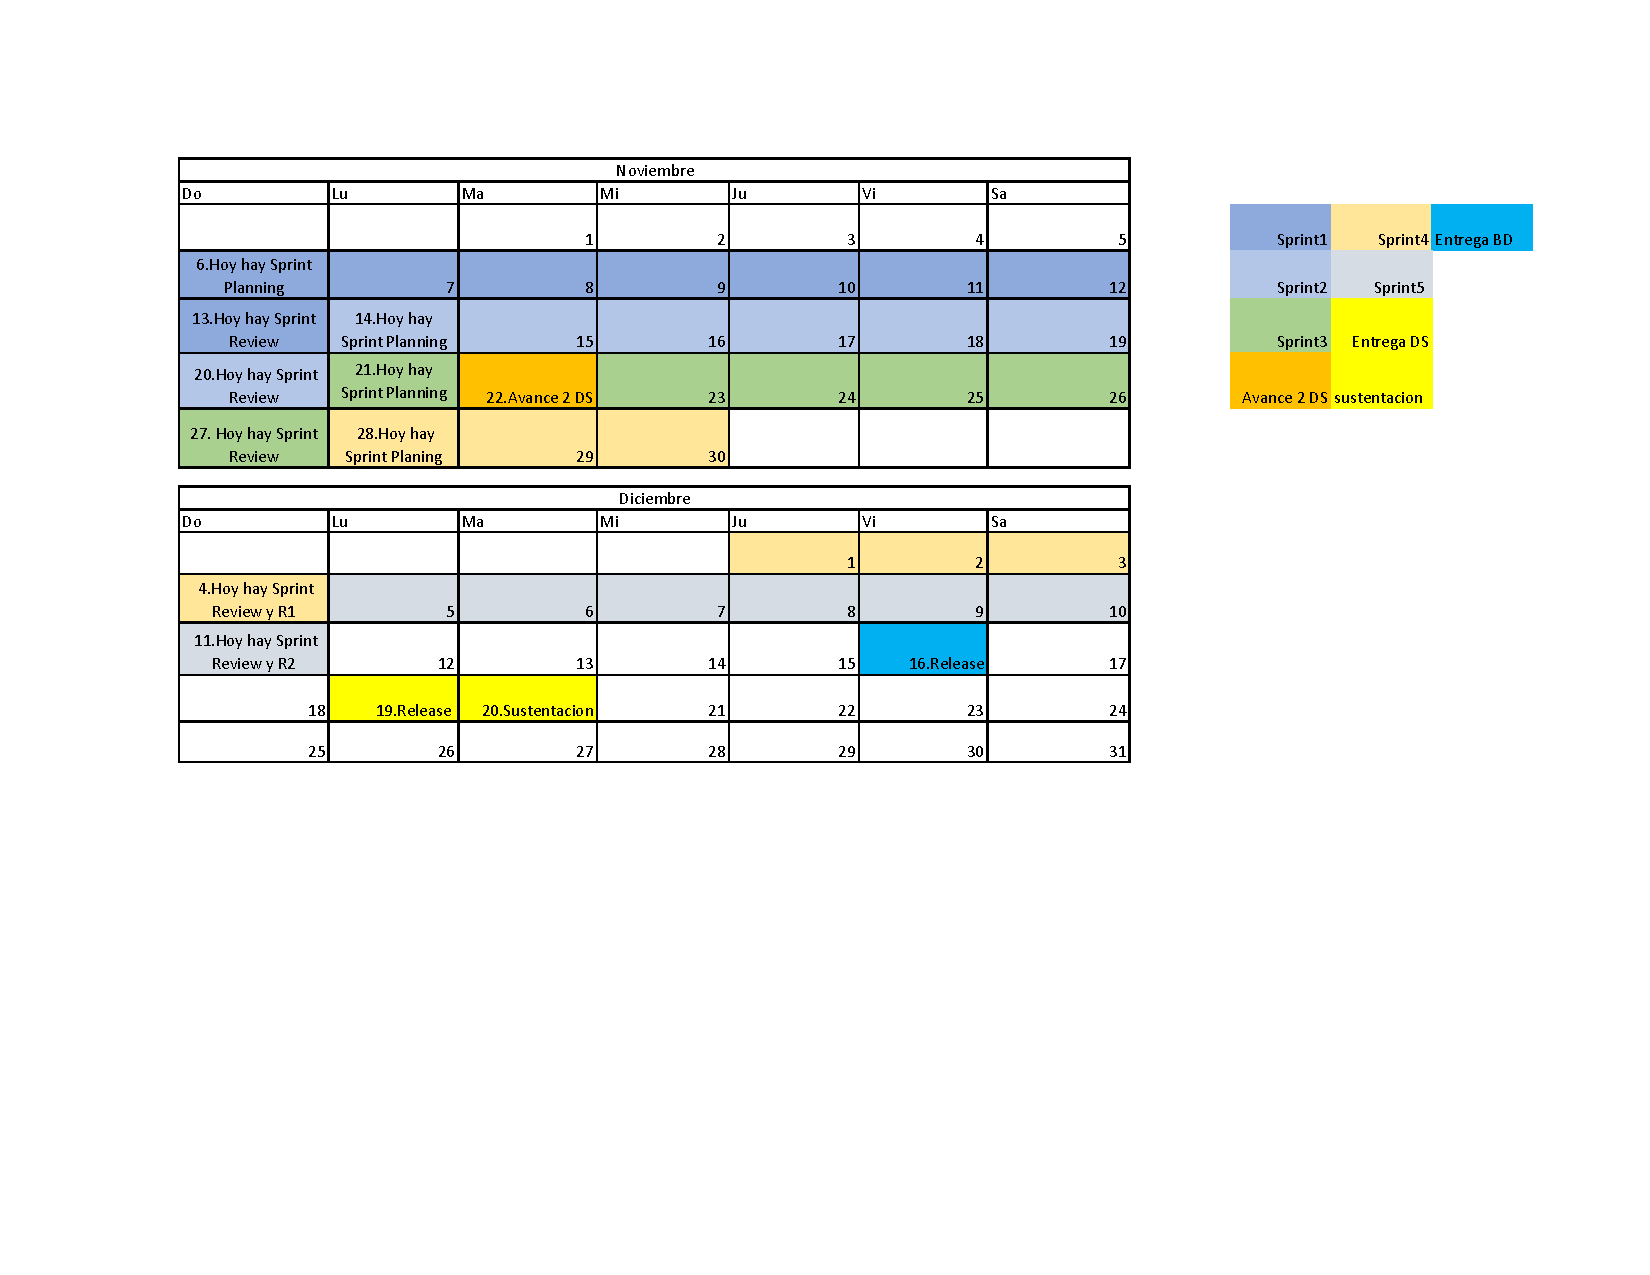
\includegraphics[width=1 \textwidth]{cronograma.pdf}\par}
\caption{Cronograma de Ceremonias Ágiles}
\end{figure}
\end{document}